\documentclass[12pt]{article}
\usepackage{geometry}
\geometry{a4paper, total={170mm,257mm},left=20mm, top=20mm, }
\usepackage[colorlinks=true,linkcolor=blue,urlcolor=black]{hyperref}
\usepackage{bookmark}
\usepackage[autostyle, english = american]{csquotes}
\usepackage[page,toc,titletoc,title]{appendix}
\usepackage{graphicx}
\begin{document}
\begin{titlepage}
\centering
\vfill
\vspace*{4\baselineskip}
{\bfseries\Large
Labtainers Instructor Guide\par
}
\vspace*{4\baselineskip}
{\bfseries
Fully provisioned cybersecurity labs\par
}
\vspace*{2\baselineskip}
\today
\vfill
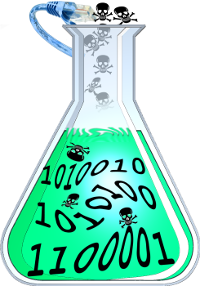
\includegraphics[width=2in]{labtainer5-sm.png}
%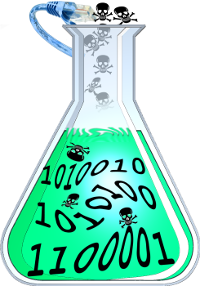
\includegraphics[width=\linewidth, scale=0.50,natwidth=200, natheight=286]{labtainer5-sm.png}
\vfill
\end{titlepage}

\section {Introduction}
This manual is intended for use by instructors who assign and/or grade
labs using Labtainers.

Labtainers provide a consistent execution environment for performing
laboratory exercises, and can include execution of several different
computers interconnected via virtual networks.  Refer to our published
papers at \url{https://nps.edu/web/c3o/labtainers} for additional information
on the use of Labtainers.  
See \ref{customizing} for information on creating and maintaining Labtainer exercises.

The easiest way to get Labtainers is to use our pre-built VM available at the Labtainer
website \url{https://nps.edu/web/c3o/virtual-machine-images}.
Note that any Linux system can be used as long as it supports Docker.

Students and instrutors can also create Labtainer VMs on the cloud using either Azure or Google cloud platforms.
See the section on ``Cloud Labtainers'' in the 
\underline{Labtainer Student Guide} for information on how to create Labtainer VMs in the cloud.

If Labtainers is to be used on a system other than the pre-built VM or the cloud,
refer to the \underline{Labtainer Student Guide} for information on
installing Labtainers.

Running Labtainers on servers, (e.g., Virtual Desktop Interface), deployments is discussed in
section \ref{servers}

\section{Assigning Labs}
Pior to assigning a lab, become familiar with it by reviewing the lab and its manual.

Student instructions for using Labtainers are in the \underline{Labtainer Student Guide}.  
Students work from the {\tt labtainer-student} directory, i.e.,
\begin{verbatim}
    cd ~/labtainer/trunk/scripts/labtainer-student
\end{verbatim}
\subsection{Selecting Labs}
Available labs are listed via the {\tt labtainer} script:
\begin{verbatim}
    labtainer
\end{verbatim}
\noindent Use the {\tt -k} option to see a list of searchable keywords, and the {\tt -f <keyword>} option to view a summary
of labs having that keyword.

Lab exercises are also organized into \textit{Labpacks}. These are ordered collections of multiple related labs that you may
wish to assign to students.  Use this command:
\begin{verbatim}
    labpack
\end{verbatim}
\noindent to view a list of Lab Packs, and provide the name of a Labpack as an argument to see a list of the labs
within a Labpack.  You may also create your own Labpacks as described in \ref{labpacks}. 

Available labs are also summerized and organized into broad categories at \url{https://nps.edu/web/c3o/labtainer-lab-summary1}.

Additional lab exercises created by instructors are available as IModules, which are listed at \url{https://nps.edu/web/c3o/imodules}.
Students can get access to those labs using:
\begin{verbatim}
    imodule <url>
\end{verbatim}
\noindent where {\tt url} is that provided on the IModules web page.

\subsection{Try the Lab}
Start a lab by providing its name as an argument to the {\tt labtainer} command.
This will typically display a link to a lab manual, or will display a lab manual in one of
the resulting virtual terminals.  You can interact with the resulting computers just as a
student would.

\section{Assessing Lab Performance}
When the student stops a lab, i.e., using {\tt stoplab}, Labtainers creates a zip file of
student artifacts (including lab reports) and then displays the path to this zip file to
the student.  This zip file has an extension of {\tt .lab} to confuse GUI-based file managers,
thus preventing click-happy students from opening the zip and submitting its internal files rather than the entire
zip (lab) file.  The easiest way for the student to forward this zip file to you is by starting
a browser on the Linux VM and either emailing you the zip file, or uploading the file
into an LMS, (e.g., Sakai).  See the \textit{Labtainers Student Guide} for a discussion of
ways in which students can forward results to the instrutor.

Collect all of the lab zip files from each student into the Labtainer transfer directory for
that lab.  On
Linux systems, e.g., the Labtainer VM appliance, the transfer directory is located at:

\begin{verbatim}
    $HOME/labtainer_xfer/<labname>
\end{verbatim}
\noindent where labname is the name of the lab.  Each lab has its own transfer directory.
Do not unzip the files.  Alternately student
assignments can be bulk-collected from a learning management system (LMS) per Appendix \ref{lms collection}
and the resulting zip  would be copied into the
transfer directory for that lab.  Again, do not unzip files and do not change the file names of zip files.
If you wish to manually review the content of the student artifact files, copy them to a different directory and
then use the {\tt unzip} command on the command line.  That utility will not be confused by the {\tt .lab} extension
and the prepended text that is intended to prevent GUI file managers from unzipping the files.

\subsection{Moving student results onto your Linux VM}
There are several ways to move student results into your transfer directory:
\begin{itemize}
\item Use the VM's browser to access email or your school's LMS system, e.g., Blackboard or Sakai.
\item Enable \textit{drag and drop} on the VM and copy the files into the transfer directory.
\item Define a shared directory as described in Appendix \ref{shared-directory}.
\item Removable media, e.g., a USB drive alternately connected to the host and the VM.
\item Enable port forwarding on the host and use {\tt scp} to move the files.
\end{itemize}

\subsection{Using gradelab}
Instructor assessment of labs takes place from the {\tt labtainer-instructor} directory, i.e.,
\begin{verbatim}
    cd ~/labtainer/trunk/scripts/labtainer-instructor
\end{verbatim}

\noindent Use the {\tt gradelab} command to assess results for a given lab:
\begin{verbatim}
    gradelab <labname>
\end{verbatim}
\noindent A table of lab results with one row per student and
a column for each goal will be displayed.  A description of the goals follows the table.
A web-based display of that data is available as described in subsection \ref{review-artifacts}.

Note that not all labs include automated assessment.  For those labs, you will see this
message:
\begin{verbatim}
  No automated assessment for this lab
\end{verbatim}
\noindent Even when no automated assessment is performed, you can still observe student performance
artifacts, e.g., the {\tt .bash\_history} file and files created by the student as described below in \ref{review-artifacts}.

By default, each time you run gradelab, a fresh grader container is created and is populated with files from the 
{\tt labtainer\_xfer} directory.   Use the {\tt -c} option to force reuse of the previous grader for that lab, in which case
any new files in the xfer directory will be added to the previous container content.
Sometimes zip files within the {\tt labtainer\_xfer} directory are corrupted.  If error messages indicate a bad zip file,
try removing it from the directory and then run gradelab again.
Use the {\tt -u } option to update your gradelab to the latest image.

Student reports (if any) are  copied into 
\begin{verbatim}
    ~/labtainer_xfer/<labname>/docs
\end{verbatim}
\noindent on the Linux host.  If LMS assignment collection is used, then student reports should
be looked for in 
\begin{verbatim}
    ~/labtainer_xfer/<labname>/reports
\end{verbatim}
\noindent which also includes reports separately uploaded into the LMS.

\subsection{Review lab artifacts}
\label{review-artifacts}
An early release of a web-based tool for viewing details of student assessment
results and student artifacts is available by use of the {\tt -w} flag with the {\tt gradelab} command.  That causes
the grader container to listen on port 8008 of the Labtainer VM.  You can then open
a browser on that VM and go to {\tt localhost:8008}.  Alternately, use your host machine's browser
by setting port forwarding on your VM, (e.g., in VirtualBox, use Machine / Settings / Network / Advanced /
Port Forwarding to set host IP 127.0.0.1:8008 to map to guest IP 0.0.0.0:8008).

The table of goals displayed in the browser includes links to details of artifacts
created by the student when performing the lab.  For example, clicking on the student name displays a table
of all timestamped result artifacts.  That page includes a \textbf{History} heading with links to the
{\tt .bash\_history} files one each container.  And it includes a table with links to files in the student home directory
and links to result files, e.g., stdout from selected commands issued by the student. 

Links within each goal table cell lead to pages whose content depends on the type of goals defined.  For example,
a goal whose value is defined by a boolean expression will lead to a table of all boolean values for each timestamp
for which results are present.

Definitions of different goal types and result types can be found in the \textit{Lab Designer Guide}.  Note that you need
not understand all of the displayed data in order to gain useful insight into student progress.  Some of the displayed information
requires an understanding of the Labtainers automated assessment configuration directives, and is made available in the displays 
primarily in support of those developing automated assessment for labs.

\subsubsection{Artifacts on the grader container}
You can view all student results, including their original artifacts by using the {\tt -d} flag
with the {\tt gradelab} command.  This results in a virtual terminal connected to a grading
container that contains all student artifacts and results.  If you have not first run the
{\tt gradelab} command without the ``-d'' option, run {\tt instructor.py} from within the
virtual terminal to cause the zip files (with a {\tt .lab} extension) to be extracted.  A student's home directory can
then be found in
\begin{verbatim}
<student email>/<lab>.<container>.student
\end{verbatim}
\noindent There you will find the {\tt .bash\_history} file along with the student-created files.
Student artifacts collected by the framework are found in 
\begin{verbatim}
<student email>/<lab>.<container>.student/.local/result
\end{verbatim}

\noindent The {\tt -d} option is also used when debugging automated assessment configuration
files.  You can create additional virtual terminals into the grading container by reissuing
the gradelab command with the {\tt -a} flag.  When you are finished, or wish to stop working, type:
\begin{verbatim}
    stoplab
\end{verbatim}


\section{Managing Labtainer Installations and Updates}
Any given Labtainers installation can be brought up to date to the latest version by using the
\begin{verbatim}
   update-labtainer.sh
\end{verbatim}
\noindent command from the {\tt labtainer-student} directory.  The current version of a Labtainer installation is seen by using:
\begin{verbatim}
   labtainer -v
\end{verbatim}
\noindent
The first time any given lab exercise is started, the latest version of that lab is automatically pulled from
the Docker Hub registry.
Note however that any given lab is not updated by the {\tt update-labtainer.sh} command once the lab has been started.  
To update a specific lab to the latest version after it has been started the previous version of that lab must be deleted
using:
\begin{verbatim}
   removelab.py <labname>
\end{verbatim}
\noindent The next time the lab is started, the latest version will be retrieved from the Docker registry.

\noindent \\If you want to update the labtainer.grader docker image (and delete the previous image and grader containers) use:
\begin{verbatim}
   gradelab -u <labname>
\end{verbatim}


\subsection{Suggestions for student workflow}
A student's work on any given lab is preserved until and unless the student restarts the lab using the ``-r'' 
option on the {\tt labtainer <labname> -r} command.  When taking a break from work on a lab, the student can
either stop the lab using {\tt stoplab}, or simply pause the VM.  However, if the student wishes to perform other
Labtainer-related work on the VM, (e.g., revisit a previous lab), they should first use {\tt stoplab} for the current
lab.  When they restart the lab, none of their work will be lost.

\subsection{Deploying without the Internet}
Labtainers pulls Docker images from Docker Hub when a student first runs any given lab.  You can deploy
Labtainers within environments that have no Internet connection by first creating your own 
VM template.  Start with the standard Labtainers VM, and run the script at 
\begin{verbatim}
   $LABTAINER_DIR/setup_scripts/pull_lab.py
\end{verbatim}
\noindent to pull images for your desired labs onto the VM.  Then replicate that VM for each user, e.g., by
exporting it as an appliance.

Note that a few labs deliberately access the Internet, e.g., the public key lab.  You can either avoid use
of those labs, or alter them to direct students to alternate network addresses.



\subsection{Deploying on servers}
\label{servers}
Labtainers can be deployed on servers and accessed by students using a web browser.  Labtainers includes
scripts for creating and accessing Labtainer VMs in the Azure and Google cloud platforms as described in
the Labtainers Student Guide.  

You can also create you own deployments, assuming you have access to suitable infrastructure and IT support.  Two general approaches are:
\begin{enumerate}
\item Virtual Desktop Infrastructure -- Use VDI products such as VMWare Horizon 
to run Labtainer VMs. In these environments, each student is allocated a VM, and that VM's desktop is seen 
by the student in the browser.  Students deliver their results to instructors by starting a browser
within the VM, e.g., to access an LMS or web-mail account.
\item \textit{Headless Labtainers} -- Labtainers are deployed as servers in a cloud and a \textit{NOVNC} desktop is 
rendered using a web browser.  Access to the Labtainer server instance is via HTTP through an SSH tunnel.
Please see \url{https://raw.githubusercontent.com/mfthomps/Labtainers/master/headless-lite/README.md} for additional information,
including a sample cloud-config file.
\end{enumerate}

\section{Customizing Labtainers}
\label{customizing}
\subsection{New and custom lab exercises}
Creating new labs and modifying existing labs is described in the \textit{Labtainers Lab Designer User Guide}.
\url{https://github.com/mfthomps/Labtainers/raw/master/docs/labdesigner/labdesigner.pdf}

That guide also describes how to use \textit{IModules} to provide your students with custom versions of the lab manuals, and how to
publish new labs so that they can be incorporated into your student's Labtainers instances, and shared
with other educators.

\subsection{Create new Labpacks}
You can organize lab exercises into your own Labapcks using the {\tt makepack} command, or with the {\tt makepackui} GUI.  
Each of these commands are run from this directory:
\begin{verbatim}
   $LABTAINER_DIR/scripts/labtainer-instructor
\end{verbatim}
\subsubsection{Command line}
Use the {\tt makepack} command, providing the name of the Labpack that you wish
to create or modify.\footnote{Do not modify other Labpacks, only modify those that you've created.}  
\begin{verbatim}
   makepack mypack1
\end{verbatim}

\noindent This results in a shell that accepts makepack commands.  Use either {\tt h} or {\tt ?} to get help.  
Note that chages to Labpacks are stored immediately, there are no save/quit options.

\subsubsection{GUI}
The {\tt makepackui} command is functionally similar to makepack, but it provides a GUI.

\subsubsection{Distributing Labpacks}
Labpacks are stored in the {\tt \$LABTAINER\_DIR/labpacks} directory.  To publish one or more Labpacks so that
they are available to your students, go to the {\tt labpacks} directory and use tar to create a tarball containing
each of your Labpacks.  For example:
\begin{verbatim}
    tar tf mypacks.tar mypack1 mypack2
\end{verbatim}
\noindent Include only the names of your custom Labpacks that you wish your students to receive.
Then post the resulting tarball on a website and provide your students with the URL.  Students will then
provide that URL to the {\tt labpack} command:
\begin{verbatim}
    labpack -a <url>
\end{verbatim}
\noindent to get access to your Labpacks.
\newpage
\begin{appendices}
%\appendix 
\pagenumbering{Alph}
\setcounter{page}{3}
\section{\\LMS Assignment Collection}
\label{lms collection}
\subsection{Sakai}
In the Sakai Assignments section, select the ``In / New'' entry for the appropriate assignment.
The resulting page should enumerate each student who has submitted an assignment.  In the upper right,
click the ``Download All'' link, and then click the ``Student submission attachment(s)'' option and
click the ``Download'' button.  Copy the resulting zip into the lab transfer directory 
on the Linux host, i.e.,
\begin{verbatim}
    ~/labtainer_xfer/<labname>
\end{verbatim}
\noindent Do not unzip the file and do not change its file name.
You can then run the {\tt gradelab <labname>} command from the {\tt labtainer-instructor} directory.
In addition to the assessment summary, any student lab reports will be available in:
\begin{verbatim}
   ~/labtainer_xfer/<labname>/reports/<student name> 
\end{verbatim}
\noindent Those reports will include any that the student separately uploaded into Sakai (it is 
important to remind students to NOT change the name of lab report documents.)

\subsection{Moodle}
See the Moodle user guide at 
\newline
\url{https://moodleuserguides.org/guides/bulk-download-assignment-submissions/}
for information on getting a bulk download, but DO NOT unzip the file.  Copy the resulting zip into the lab transfer directory 
on the Linux host, i.e.,
\begin{verbatim}
    ~/labtainer_xfer/<labname>
\end{verbatim}
\noindent Do not unzip the file and do not change its file name.
You can then run the {\tt gradelab <labname>} command from the {\tt labtainer-instructor} directory.
In addition to the assessment summary, any student lab reports will be available in:
\begin{verbatim}
   ~/labtainer_xfer/<labname>/reports/<student name> 
\end{verbatim}
\noindent Those reports will include any that the student separately uploaded into Moodle (it is 
important to remind students to NOT change the name of lab report documents.)

\subsection{Other LMS}
Send me a sample of the bulk download file from other LMS systems and we'll roll it into a future Labtainers release. (mfthomps at nps.edu)

\newpage
\section{Defining shared folders}
\label{shared-directory}
It is often more convenient for instructors to gather student zip files on the computer that hosts a Labtainers
VM rather than on the VM.  For example, email clients and/or LMS interfaces may run more easily on the host than
they do on the VM.  One way that this can be achieved is by defining a shared folder for use by the VM guest, as follows:
\begin{itemize}
\item Pick a directory on your host that you will share with the VM. Somewhere within that directory create a
{\tt labtainer\_xfer} subdirectory.
\item Make that directory accessible by anyone on your host machine.  
\item Define a shared folder for your guest VM, e.g., on VirtualBox, use Machine / Settings / Shared folders, map it
to your selected directory.  
\item On VirtualBox, ensure your user ID is within the vboxsf group, and reboot.
\begin{verbatim}
    sudo usermod -G vboxsf -a $USER
    sudo reboot
\end{verbatim}
\item On the virtual machine, identify the path to the {\tt labtainer\_xfer} directory in the shared folder.  For example,
if you shared a directory called {\tt mydir} on VirtualBox, that might be found at {\tt /media/sf\_mdir/labtainer\_xfer}.
\item From the \$HOME directory on the virtual machine, remove the {\tt labtainer\_xfer} directory and replace it with
a symbolic link to the shared {\tt labtainer\_xfer} directory, e.g.,
\begin{verbatim}
   cd 
   ln -s /media/sf_mydir/labtainer_xfer
\end{verbatim}
\noindent depending on where you created the new {\tt labtainer\_xfer} directory within the shared folder.
\item Now place student zip files on the host within the {\tt labtainer\_xfer/<labname>} directory.  Note
the lab subdirectory will be created when you start the lab to run it yourself -- or you can create it manually.
\end{itemize}
\end{appendices}
\end{document}
